\documentclass[11pt,a4paper]{article}
\usepackage[czech]{babel}
\usepackage[utf8]{inputenc}
\usepackage[T1]{fontenc}
\usepackage{times}
\usepackage[text={17cm,24cm},left=2cm,top=2.5cm]{geometry}
\usepackage{xcolor,colortbl}
\usepackage{color}
\newcommand{\myuv}[1]{\quotedblbase #1\textquotedblleft}
\usepackage{graphicx}
\graphicspath{ {images/} }



\begin{document}

%%%%%%%%%%%%%%%%%%%%%%%%%%%%%%%%%%%%%%%%%%%%%%%%%%%%%%%%%%%%%%%%%%%%%%%%%%
%%%%%%%%%%					Titulná strana						%%%%%%%%%%
%%%%%%%%%%%%%%%%%%%%%%%%%%%%%%%%%%%%%%%%%%%%%%%%%%%%%%%%%%%%%%%%%%%%%%%%%%
\begin{titlepage}

	\begin{center}
		{\textbf{\Huge\textsc{Vysoké učení technické v~Brně}}} \\
		\bigskip
		{\huge\textsc{Fakulta informačních technologií}}
		\bigskip
		
\includegraphics[scale=0.15]{logo}
		\huge{Dokumentácia k projektu do predmetu  IFJ a IAL} \\
		\medskip
		{\textbf{\Huge{Implementácia prekladača imperatívneho jazyka IFJ17}}} \\
		\medskip
		\huge{Tím 8, varianta II} \\
		\medskip
		\today
	\end{center}

\vfill

\noindent
\Large{\textbf{Kristián Liščinský}\hfill (xlisci01,) 25\%\\\textbf{Matúš Liščinský}\hfill (xlisci02), 25\% \\\textbf{Vladimír Marcin}\hfill (xmarci00), 25\% \\ \textbf{Šimon Stupinský}, vedúci\hfill  (xstupi10), 25\%}
\indent
\end{titlepage}

%%%%%%%%%%%%%%%%%%%%%%%%%%%%%%%%%%%%%%%%%%%%%%%%%%%%%%%%%%%%%%%%%%%%%%%%%%
%%%%%%%%%%					    Obsah							%%%%%%%%%%
%%%%%%%%%%%%%%%%%%%%%%%%%%%%%%%%%%%%%%%%%%%%%%%%%%%%%%%%%%%%%%%%%%%%%%%%%%
\tableofcontents
\newpage
%%%%%%%%%%%%%%%%%%%%%%%%%%%%%%%%%%%%%%%%%%%%%%%%%%%%%%%%%%%%%%%%%%%%%%%%%%
%%%%%%%%%%					    Úvod							%%%%%%%%%%
%%%%%%%%%%%%%%%%%%%%%%%%%%%%%%%%%%%%%%%%%%%%%%%%%%%%%%%%%%%%%%%%%%%%%%%%%%
\section{Úvod}

Dokumentácia popisuje implementáciu prekladača imperatívneho jazyka IFJ17. Zvolili sme si variantu II, ktorá obsahovala implementáciu tabuľky symbolov pomocou tabuľky s rozptýlenými položkami. Implementáciu sme rozdelili do 3 hlavných častí, pričom každej z nich bude venovaná samostatná kapitola.
\begin{itemize}
	\item lexikálna analýza
	\item synktatická a sémantická analýza
		\begin{itemize}
			\item synktatická analýza (bez spracovania výrazov)
			\item synktatická analýza výrazov
		\end{itemize}
	\item generovanie vnútorného kódu
\end{itemize}
Dokumentácia taktiež zahrňuje 3 prílohy, ktoré obsahujú diagram konečného automatu, popisujúci lexikálny analyzátor, LL gramatiku a precedenčnú tabuľku.

%%%%%%%%%%%%%%%%%%%%%%%%%%%%%%%%%%%%%%%%%%%%%%%%%%%%%%%%%%%%%%%%%%%%%%%%%%
%%%%%%%%%%					    1. Kapitola						%%%%%%%%%%
%%%%%%%%%%%%%%%%%%%%%%%%%%%%%%%%%%%%%%%%%%%%%%%%%%%%%%%%%%%%%%%%%%%%%%%%%%
\section{Jazyk IFJ17}
Jazyk IFJ17 je zjednodušenou podmnožinou jazyka FreeBASIC, ktorý stavia na legendárnom jazyku BASIC, je staticky typovaný
imperativní jazyk. V jazyku IFJ17 nezáleží na veľkosti písmen u identifikátorov a kľúčových slov, je teda case\,-\,insensitive.
Je možné pracovať s celočíselným, alebo desatinným literálom v základnom a exponenciálnom tvare. Zároveň je tiež možné využívať aj reťazcový literál, ktorý môže obsahovať escape sekvencie zadané v dekadickom tvare. Podporovanými dátovými typmi jazyka IFJ17 sú typy Integer, Double a String a zároveň jazyk podporuje ako riadkové, tak aj blokové komentáre. Výrazy sú tvorené pomocou termov, zátvoriek a binárnych aritmetických, reťazcových a relačných operátoroch. 


%%%%%%%%%%%%%%%%%%%%%%%%%%%%%%%%%%%%%%%%%%%%%%%%%%%%%%%%%%%%%%%%%%%%%%%%%%
%%%%%%%%%%					    2. Kapitola						%%%%%%%%%%
%%%%%%%%%%%%%%%%%%%%%%%%%%%%%%%%%%%%%%%%%%%%%%%%%%%%%%%%%%%%%%%%%%%%%%%%%%
\section{Štruktúra projektu}
	\subsection{Lexikálna analýza}

	Lexikálna analýza je činnosť, ktorú vykonáva takzvaný lexikálny analyzátor (scanner). Je to vstupná a najjednoduchšia časť prekladača. Lexikálny analyzátor rozdeľuje vstupnú postupnosť znakov, ktoré reprezentujú zdrojový program, na jednotlivé lexikálne jednotky - lexémy \footnote{https://www.fit.vutbr.cz/study/courses/IFJ/private/prednesy/Ifj05-anim-cz.pdf}. Lexémy sú reprezentované vo forme tokénov a tie sú nasledne poskytované synktatickému analyzátoru. Jednotlivé tokeny generované lexikálnou analýzou sú implementované ako dvojice (sym, atr), kde sym je meno (identifikácia) symbolu a atr predsavuje prípadný atribut symbolu. U symbolov bez atribútu je atr prázdne\footnote{https://cs.wikipedia.org/wiki/Lexikální\_analýza}. Úlohou lexikálneho analyzátora je taktiež zbaviť zdrojový program bielych znakov a komentárov. V praxi je implementovaný pomocou konečného automatu. Diagram konečného automatu si môžte pozrieť v priloženej prílohe (7.2). V prípade, že načítame niečo, čo nezapadá do pravidiel programovacieho jazyka IFJ17 nastane lexikálna chyba.

	\subsection{Synktatická a sémantická analýza}
		\subsubsection{Synktatická analýza (bez spracovania výrazov)}

		Syntaktický analyzátor (parser) kontroluje množinu pravidiel, ktorá určuje prípustné konštrukcie daného jazyka. Syntaktická analýza je 
		implementovaná rekurzívnym zostupom, ktorý je riadený pravidlami LL-gramatiky uvedenými v prílohe (7.1). Terminálne symboly predstavujú 
		tokeny ktoré sú na požiadanie vrátené lexikálnym analyzátorom. Na základe prijatých tokenov syntaktický analyzátor simuluje tvorbu 
		derivačného stromu. Ak sa nepodarí nasimulovať derivačný strom, jedná sa o syntaktickú chybu a analýza sa ukončí.

		Spolu so syntaktickou analýzou je súčasne vykonávaná aj semántická analýza. Pri definícii alebo deklarácii funkcie sa do globálnej tabuľky 
		symbolov uloží dátová štruktúra reprezentujúca danú funkciu (v jazyku IFJ17 sú v globálnej tabuľke symbolov uložené iba funkcie) a súčasne 
		sa vykonávajú semantické kontroly (napr.: či sa nejedná o redefiníciu funkcie apod.). V prípade definície funkcie sa následne spracováva 
		telo funkcie. Priamo pri rekurzívnom zostupe sa vykonávajú všetky potrebné sémantické kontroly a napĺňa sa lokálna tabuľka symbolov príslušnej funkcie. 
		Keď pri spracovávaní zdrojového súboru parser narazí na výraz, riadenie je predané modulu expr (volanie funkcie expression(\dots)), ktorý 
		pomocou precedenčnej analýzy skontroluje správnosť výrazu a vyvolá potrebné sémantické kontroly a vráti riadenie späť parseru.

		\subsubsection{Synktatická analýza výrazov}

		Pre spracovanie výrazov sme podľa zadania použili precedenčnú syntaktickú analýzu, riadenú precedenčnou tabuľkou. Modul vykonávajúci spracovanie výrazov, je volaný syntaktickým analyzátorom pri dvoch situáciách. Tou prvou je samotné spracovanie výrazov a druhou je volanie užívateľských a vstavaných funkcií.
		
		Parser načítava postupnosť tokenov a podľa pravidiel v LL-gramatike, v ktorých sa vyskytuje výraz, alebo volanie funkcie, predáva riadenie precedenčnej analýze. Vstupom tejto analýzy je postupnosť tokenov získaná lexikálnym analyzátorom a výstupom je postupnosť inštrukcií, ktoré sú zároveň vstupom pre dodaný interpret.
		
		Spracovanie výrazov riadené precedečnou tabuľkou (príloha 7.3) prebieha v dvoch krokoch. V prvom kroku je kontrolovaná správna postupnosť tokenov, ktoré sú prípustné v rámci syntaxe. V kladnom prípade, je výraz pomocou zásobníkovej štruktúry prevedený z infixovej notácie na výhodnú postfixovu. V druhom kroku je postfixová notácia prevádzaná na príslušné inštrukcie, zabezpečujúce vyhodnotenie výrazu. V tomto kroku zároveň prebieha kontrola typovej kompatibility operandov a prípadne sú generovane inštrukcie implicitného pretypovania.
		
		Volanie funkcií je obsiahnuté v kontrole typovej kompatibility parametrov a ich počtu. Na záver je kontrolovaná typová kompatibilita návratového typu volanej funkcie s typom premennej, do ktorej by mala byť priradená návratová hodnota funkcie.


	\subsection{Generovanie vnútorného kódu}

	Počas priebehu vykonávania syntaktickej a sémantickej analýzy sa generujú ekvivalentné inštrukcie kódu jazyka IFJcode17.
	Postupne sa tak inštrukciami plní jedna globálna inštrukčná páska implementovaná ako jednosmerne viazaný zoznam.
	Celá inštrukčná páska sa vypíše na štandardný výstup iba v prípade lexikálnej, syntaktickej i sémantickej správnosti zdrojového textu v jazyku IFJ17.

%%%%%%%%%%%%%%%%%%%%%%%%%%%%%%%%%%%%%%%%%%%%%%%%%%%%%%%%%%%%%%%%%%%%%%%%%%
%%%%%%%%%%					    3. Kapitola						%%%%%%%%%%
%%%%%%%%%%%%%%%%%%%%%%%%%%%%%%%%%%%%%%%%%%%%%%%%%%%%%%%%%%%%%%%%%%%%%%%%%%
\section{Riešenie vybraných algoritmov z pohľadu predmetu IAL}
	
	\subsection{Zásobník}
	Zásobník je implementovaný pomocou dátovej štruktúry jednosmerného zoznamu. Štruktúra zásobníka obsahuje ukazateľ na položku zásobníka ktorá je aktuálne na vrchole zásobníka. Položka zásobníka predstavuje ukazateľ na dátový typ void a ukazateľ na nasledujúci prvok.

	To že sme sa položku zásobníka rozhodli implementovať pomocou ukazateľa na dátový typ void, bolo ovplyvnené tým, že táto voľba umožňuje široké využitie zásobníka. Samotný zásobník vhodne využívame vo viacerých prípadoch. Prvým z nich je prevádzanie výrazov na postfixovu notáciu, pri ktorej využívame dva zásobníky. Prvý pre tvorbu výsledného výrazu a druhý pre pomocné ukladanie operátorov a zátvoriek podľa ich priorít. Zásobník je tiež využívaný pri tvorbe inštrukcií pre vyhodnotenie výrazov a tiež pre ukladanie parametrov funkcie, kvôli uchovaniu príslušného poradia.
	
	Špeciálne využitie zásobníka predstavuje modul pre uvoľnenie alokovanej pamäte počas behu programu. Ukazatele na alokovanú pamäť sa ukladajú na zásobník a pred ukončením behu programu sú tieto ukazetele korektne uvoľnené. Tento modul ma tak podobnú funkčnosť ako známy garbage collector.

	\subsection{Tabuľka s rozptýlenými položkami}
	Tvorí základ tabuľky symbolov. Slúži na ukladanie dvojice kľúč-hodnota. Jej výhodou je rýchlosť vyhľadávania položiek. Základom je pole 
	ukazateľov na jednotilivé položky. Jedna položka obsahuje obsahuje svoj kľúč, data a ukazateľ na ďalšiu položku, aby mohli byť zreťazené 
	v jednosmerne viazanom zozname synonym.

	V našom prípade data jednej položky predstavujú ukazateľ na štruktúru reprezentujúcu 
	premennú/funkciu. Dobrá hashovacia funkcia má zásadný vplyv na výkon tabuľky. Nami vybraná hashovacia funkcia, ktorú sme použili, je 
	uvedená v referenciách \footnote{http://www.cse.yorku.ca/~oz/hash.html}(varianta sdbm). V prípade ideálnej hashovacej funkcie je čas prístupu k položkám konštantný pričom v prípade 
	konfliktu sa čas nájdenia položky predlží o dobu prehľadania zoznamu synonym.
	V našom programe sa nachádza jedna globálna tabuľka symbolov v ktorej sú uložené informácie o funkciách pričom každá funkcia ma svoju 
	vlastnú tabuľku symbolov, ktorá obsahuje informácie o parametroch/lokálnych premenných funkcie. 
	Tabuľka symbolov je implementovaná v súboroch symtable.c a symtable.h.


	

%%%%%%%%%%%%%%%%%%%%%%%%%%%%%%%%%%%%%%%%%%%%%%%%%%%%%%%%%%%%%%%%%%%%%%%%%%
%%%%%%%%%%					    4. Kapitola						%%%%%%%%%%
%%%%%%%%%%%%%%%%%%%%%%%%%%%%%%%%%%%%%%%%%%%%%%%%%%%%%%%%%%%%%%%%%%%%%%%%%%
\section{Vývoj}
Tím o 4 ľuďoch už vyžaduje opatrenia, aby bol vývoj riadený, aby každý vedel, čo treba robiť a
čo robia ostatní. Tieto opatrenia bolo potrebné zaviesť hneď na začiatku, ešte predtým ako sa
začne vývojový cyklus.

	\subsection{Rozdelenie práce}
		\begin{itemize}
		\item 	\textbf{Kristián Liščinský:} lexikálna analýza, dokumentácia, testovanie
		\item 	\textbf{Matúš Liščinský:} generovanie kódu, pomocné moduly pre pre prácu s reťazcami, garbage collector, testovanie 
		\item 	\textbf{Vladimír Marcin:} syntaktická analýza bez spracovavania výrazov, sémantické kontroly, návrh tabuľky symbolov, testovanie
		\item 	\textbf{Šimon Stupinský} syntaktická analýza so spracovavaním výrazov, sémantické kontroly, implementácia zásobníka, autmatické testy
		\end{itemize}

	\subsection{Komunikácia a použité prostriedky}
	Komunikácia nášho tímu prebiehala prevažne osobne v pravidelných intervaloch, ktoré sa s blížiacím príchodom dňa odovzdania znižovali. Okrem toho sme tiež využívali online komunikáciu v podobe skupinového chatu na facebooku.

	Keďže práca celého tímu bola závislá na jedných a tých istých súboroch, pre väčší komfort sme sa rozhodli využiť distribuovaný verzovací systém git.

%%%%%%%%%%%%%%%%%%%%%%%%%%%%%%%%%%%%%%%%%%%%%%%%%%%%%%%%%%%%%%%%%%%%%%%%%%
%%%%%%%%%%					    Záver							%%%%%%%%%%
%%%%%%%%%%%%%%%%%%%%%%%%%%%%%%%%%%%%%%%%%%%%%%%%%%%%%%%%%%%%%%%%%%%%%%%%%%
\section{Záver}

Projekt bol naším prvým tímovým projektom, prvykrát sme museli vzájomne komunikovať a konzultovať jednotlivé možnosti implementácie a zmeny v zdrojových kódoch. Počas práce na ňom sme si rozšírili svoje znalosti a získali sme skúsenosti s prácou na rozsiahlejšiom projekte a prácou v tíme. Oboznámili sme sa s náročnosťou rôznych fáz tvorby projektu od návrhu až po testovanie. Využili sme možnosť pokusného odovzdania, ktoré nám pomohlo získať predstavu o stave jednotlivých častí nášho projektu. Na základe týchto informácií sme sa vedeli zamerať na slabšie miesta našej implementácie. Snažili sme sa vytvoriť program, ktorý bude plne vyhovovať zadaniu. Na konci sme dospeli k názoru, že práca na projekte nás posunula vpred nielen v programátorskom, ale aj ľudskom smere.

	\subsection{Metriky}
	\begin{itemize}
		\item 	Počet súborov: \textbf{23}
		\item 	Počet riadkov zdrojového kódu: \textbf{2493}
		\item 	Počet Git commitov: \textbf{108}
	\end{itemize}
\newpage
%%%%%%%%%%%%%%%%%%%%%%%%%%%%%%%%%%%%%%%%%%%%%%%%%%%%%%%%%%%%%%%%%%%%%%%%%%
%%%%%%%%%%					    Prílohy					    	%%%%%%%%%%
%%%%%%%%%%%%%%%%%%%%%%%%%%%%%%%%%%%%%%%%%%%%%%%%%%%%%%%%%%%%%%%%%%%%%%%%%%
\section{Prílohy}
	
	\subsection{LL gramatika}
	\begin{center}
	\begin{tabular}{|c||c|c|c|}
	\hline
	1&<prog> &->& <declare-function> EOL <prog>\\
	\hline
	2&<prog> &->& <define-function> EOL <prog>\\
	\hline
	3&<prog> &->& <main-function>\\
	\hline
	4&<prog> &->& EOL <prog>\\
	\hline
	5&<declare-function> &->& Declare Function id (<param-list>) As <data-type>\\
	\hline
	6&<define-function> &->& Function id (<param-list>) As <data-type> EOL <function-element> \\
	&&&End Function| Function\\
	\hline
	7&<main-function> &->& Scope EOL <function-element> End Scope\\
	\hline
	8&<function-element> &->& epsilon\\
	\hline
	9&<function-element> &->& Dim id As <data-type> <value> EOL <function-element>\\
	\hline
	10&<function-element> &->& <element-list>\\
	\hline
	11&<element-list> &->& <statement> <function-element>\\
	\hline
	12&<statement> &->& EOL\\
	\hline
	13&<statement> &->& id = <call-assign> EOL\\
	\hline
	14&<statement> &->& Print <E> ; <exp-to-print> EOL\\
	\hline
	15&<statement> &->& Input id EOL\\
	\hline
	16&<statement> &->& Return <E> EOL\\
	\hline
	17&<statement> &->& Do While <E> EOL <stat-list> Loop EOL\\
	\hline
	18&<statement> &->& If <E> Then EOL <stat-list> <else-branch> End If EOL\\
	\hline
	19&<value> &->& epsilon\\
	\hline
	20&<value> &->& = <E>\\
	\hline
	21&<else-branch> &->& epsilon\\
	\hline
	22&<else-branch> &->& Else EOL <stat-list>\\
	\hline
	23&<stat-list> &->& <statement> <stat-list>\\
	\hline
	24&<stat-list> &->& epsilon\\
	\hline
	25&<exp-to-print> &->& <E> ; <exp-to-print>\\
	\hline
	26&<exp-to-print> &->& epsilon\\
	\hline
	27&<call-assign> &->& <E>\\
	\hline
	28&<call-assign> &->& id(<param-value>)\\
	\hline
	29&<param-value> &->& epsilon\\
	\hline
	30&<param-value> &->& <E> <next-param-value>\\
	\hline
	31&<next-param-value> &->& , <E> <next-param-value>\\
	\hline
	32&<next-param-value> &->& epsilon\\
	\hline
	33&<param-list> &->& <param> <next-param>\\
	\hline
	34&<next-param> &->& , <param> <next-param>\\
	\hline
	35&<param-list> &->& epsilon\\
	\hline
	36&<next-param> &->& epsilon\\
	\hline
	37&<param> &->& id As <data-type>\\
	\hline
	38&<data-type> &->& Integer\\
	\hline
	39&<data-type> &->& String\\
	\hline
	40&<data-type> &->& Double\\
	\hline

	\end{tabular}
	\end{center}

	\begin{figure}
		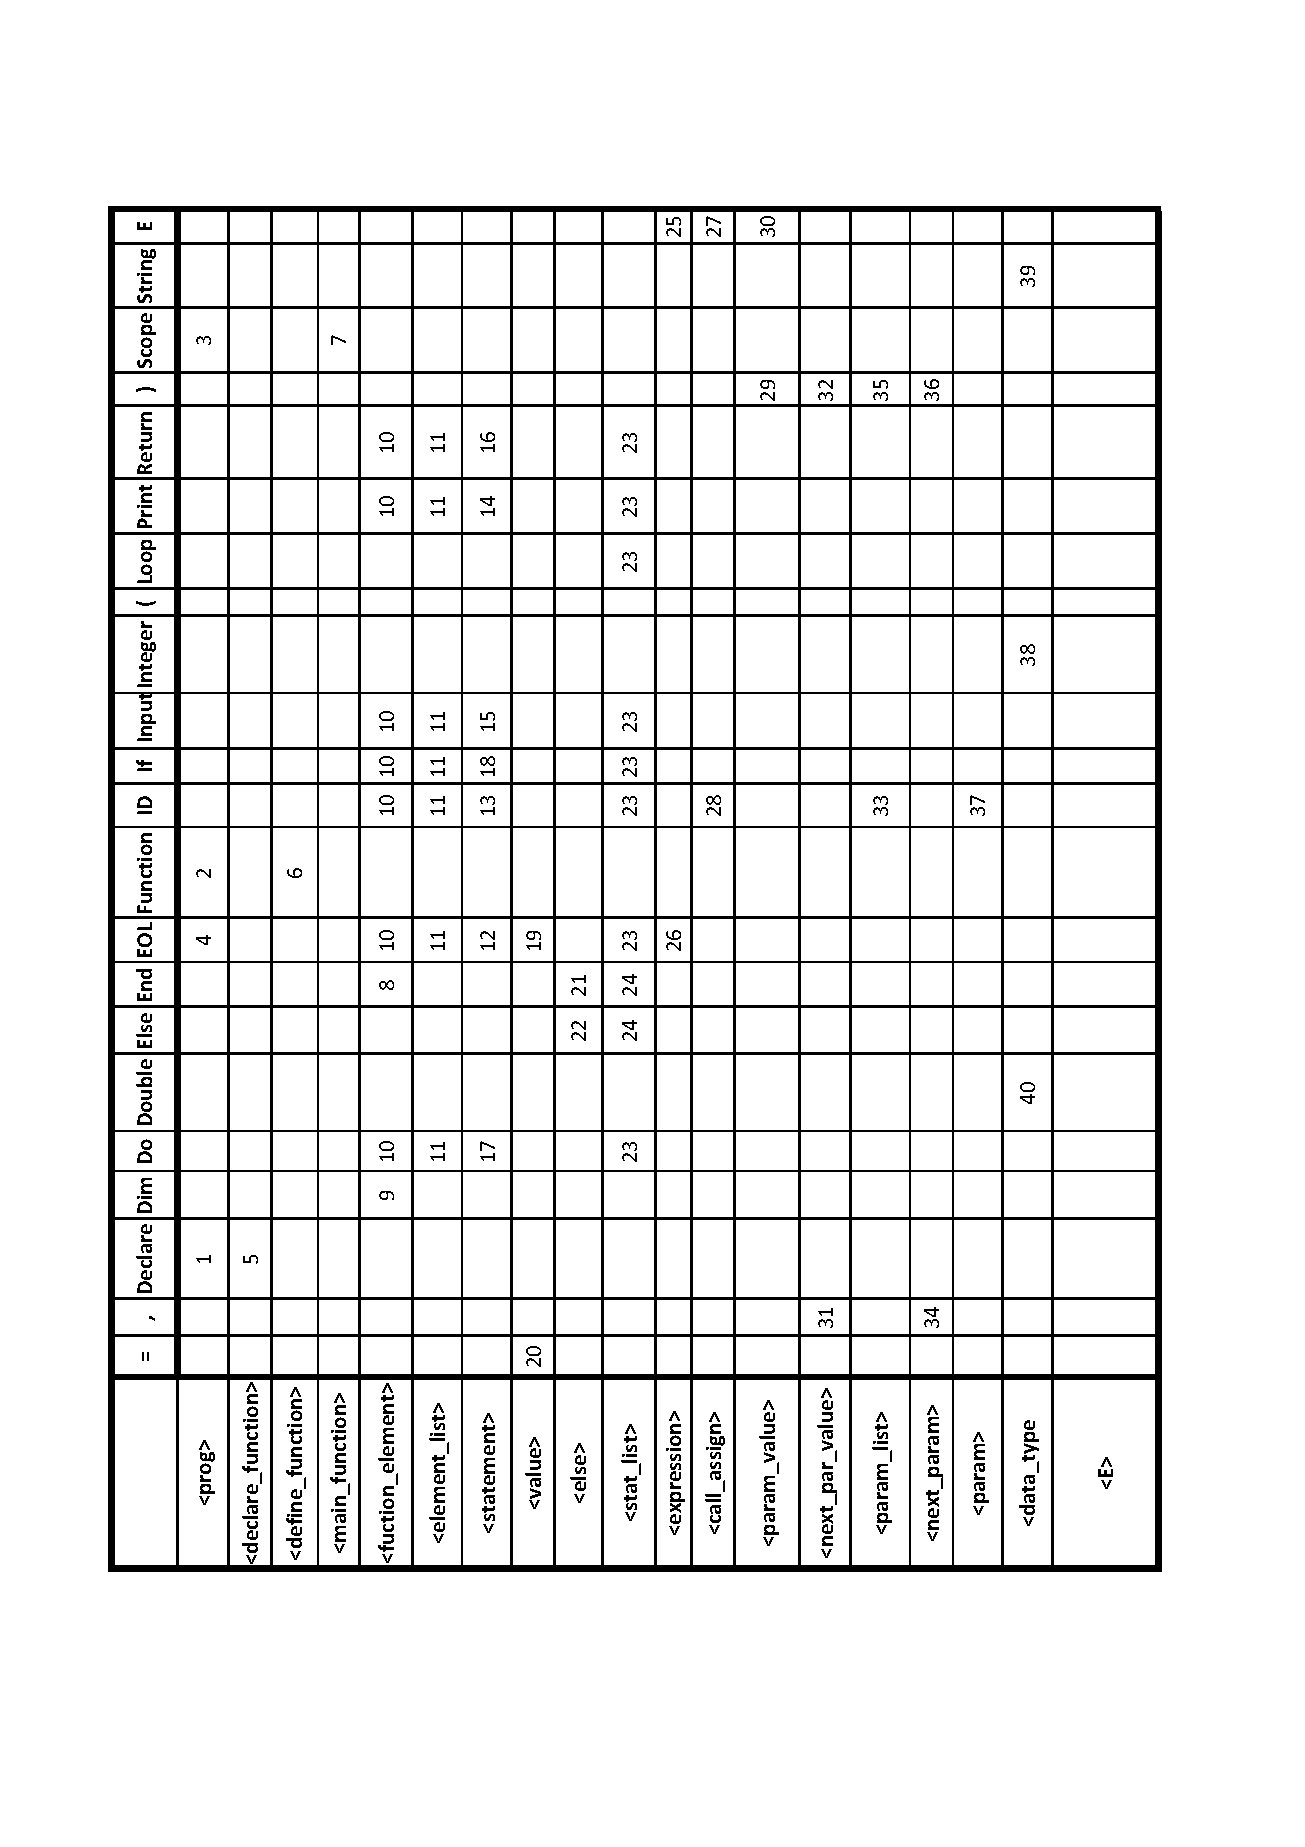
\includegraphics[scale=0.8]{LL_table}
	\end{figure}

	\begin{figure}
	\subsection{Diagram konečného automatu lexikálneho analyzátora}
		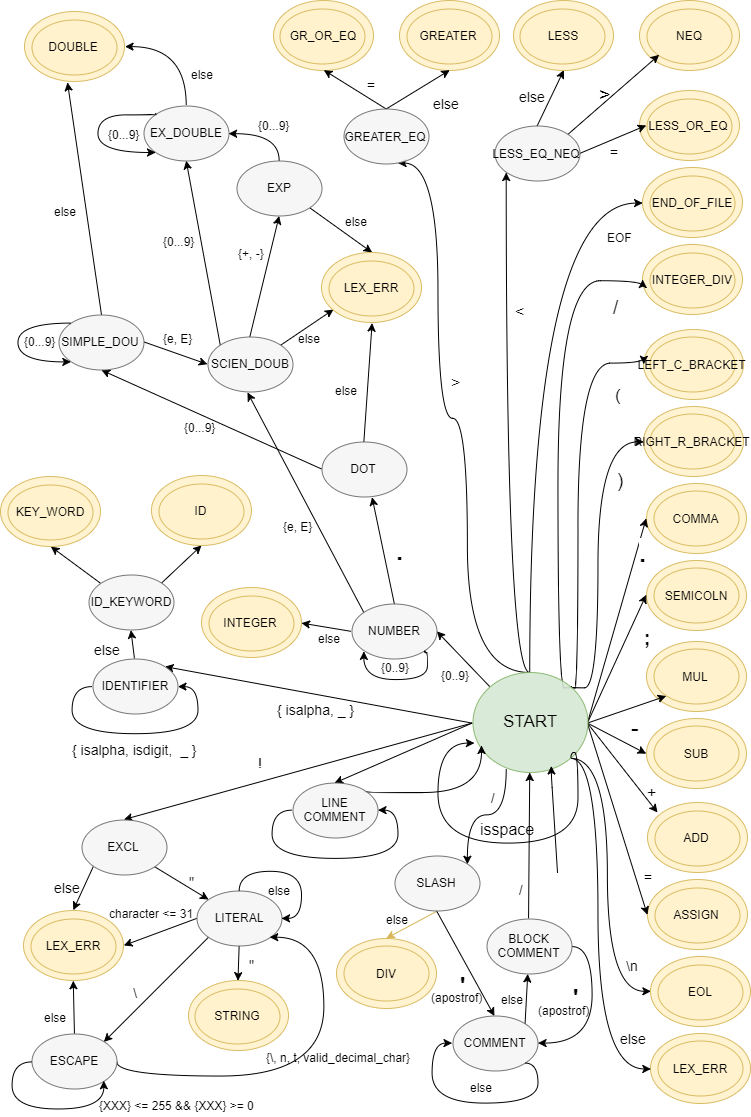
\includegraphics[scale=0.65]{scanner}
	\end{figure}
	

	\subsection{Precedenčná tabuľka}
	\begin{center}
	\begin{LARGE}
	\begin{tabular}{|c||c|c|c|c|c|c|c|c|c|c|c|c|c|c|c|c|}
	\hline
	\rowcolor{green}
	&+&-&*&/&(&)&\textbackslash&<&>&<=&>=&=&<\,>&id&lit&\$\\
	\hline
	\hline
	\cellcolor{green}+&\color{red}>&\color{red}>&\color{blue}<&\color{blue}<&\color{blue}<&\color{red}>&\color{blue}<&\color{red}>&\color{red}>&\color{red}>&\color{red}>&\color{red}>&\color{red}>&\color{blue}<&\color{blue}<&\color{red}>\\
	\hline
	\cellcolor{green}-&\color{red}>&\color{red}>&\color{blue}<&\color{blue}<&\color{blue}<&\color{red}>&\color{blue}<&\color{red}>&\color{red}>&\color{red}>&\color{red}>&\color{red}>&\color{red}>&\color{blue}<&\color{blue}<&\color{red}>\\
	\hline
	\cellcolor{green}*&\color{red}>&\color{red}>&\color{red}>&\color{red}>&\color{blue}<&\color{red}>&\color{red}>&\color{red}>&\color{red}>&\color{red}>&\color{red}>&\color{red}>&\color{red}>&\color{blue}<&\color{blue}<&\color{red}>\\
	\hline
	\cellcolor{green}/&\color{red}>&\color{red}>&\color{red}>&\color{red}>&\color{blue}<&\color{red}>&\color{red}>&\color{red}>&\color{red}>&\color{red}>&\color{red}>&\color{red}>&\color{red}>&\color{blue}<&\color{blue}<&\color{red}>\\
	\hline
	\cellcolor{green}(&\color{blue}<&\color{blue}<&\color{blue}<&\color{blue}<&\color{blue}<&\color{green}=&\color{blue}<&\color{blue}<&\color{blue}<&\color{blue}<&\color{blue}<&\color{blue}<&\color{blue}<&\color{blue}<&\color{blue}<&\\
	\hline
	\cellcolor{green})&\color{red}>&\color{red}>&\color{red}>&\color{red}>&&\color{red}>&\color{red}>&\color{red}>&\color{red}>&\color{red}>&\color{red}>&\color{red}>&\color{red}>&&&\color{red}>\\
	\hline
	\cellcolor{green}\textbackslash&\color{red}>&\color{red}>&\color{blue}<&\color{blue}<&\color{blue}<&\color{red}>&\color{red}>&\color{red}>&\color{red}>&\color{red}>&\color{red}>&\color{red}>&\color{red}>&\color{blue}<&\color{blue}<&\color{red}>\\
	\hline
	\cellcolor{green}<&\color{blue}<&\color{blue}<&\color{blue}<&\color{blue}<&\color{blue}<&\color{red}>&\color{blue}<&&&&&&&\color{blue}<&\color{blue}<&\color{red}>\\
	\hline
	\cellcolor{green}>&\color{blue}<&\color{blue}<&\color{blue}<&\color{blue}<&\color{blue}<&\color{red}>&\color{blue}<&&&&&&&\color{blue}<&\color{blue}<&\color{red}>\\
	\hline
	\cellcolor{green}<=&\color{blue}<&\color{blue}<&\color{blue}<&\color{blue}<&\color{blue}<&\color{red}>&\color{blue}<&&&&&&&\color{blue}<&\color{blue}<&\color{red}>\\
	\hline
	\cellcolor{green}>=&\color{blue}<&\color{blue}<&\color{blue}<&\color{blue}<&\color{blue}<&\color{red}>&\color{blue}<&&&&&&&\color{blue}<&\color{blue}<&\color{red}>\\
	\hline
	\cellcolor{green}=&\color{blue}<&\color{blue}<&\color{blue}<&\color{blue}<&\color{blue}<&\color{red}>&\color{blue}<&&&&&&&\color{blue}<&\color{blue}<&\color{red}>\\
	\hline
	\cellcolor{green}<\,>&\color{blue}<&\color{blue}<&\color{blue}<&\color{blue}<&\color{blue}<&\color{red}>&\color{blue}<&&&&&&&\color{blue}<&\color{blue}<&\color{red}>\\
	\hline
	\cellcolor{green}id&\color{red}>&\color{red}>&\color{red}>&\color{red}>&&\color{red}>&\color{red}>&\color{red}>&\color{red}>&\color{red}>&\color{red}>&\color{red}>&\color{red}>&&&\color{red}>\\
	\hline
	\cellcolor{green}lit&\color{red}>&\color{red}>&\color{red}>&\color{red}>&&\color{red}>&\color{red}>&\color{red}>&\color{red}>&\color{red}>&\color{red}>&\color{red}>&\color{red}>&&&\color{red}>\\
	\hline
	\cellcolor{green}\$&\color{blue}<&\color{blue}<&\color{blue}<&\color{blue}<&\color{blue}<&&\color{blue}<&\color{blue}<&\color{blue}<&\color{blue}<&\color{blue}<&\color{blue}<&\color{blue}<&\color{blue}<&\color{blue}<&\\
	\hline
	
	\end{tabular}
	\end{LARGE}
	\end{center}

\end{document}